%%%%%%%%%%%%%%%%%%%%%%%%%%%%%%%%%
% 6CCS3PRJ Final Year Individual Project Report
%%%%%%%%%%%%%%%%%%%%%%%%%%%%%%%%%
\documentclass[11pt]{informatics-report}
\usepackage{color}
\usepackage[square,sort,comma,numbers]{natbib} %References
\usepackage{graphicx}
\usepackage{hyperref}

%%%%%%%%%%%%%%%%%%%%%%%%%%%%%%%%%
% Front Matter - project title, name, supervisor name and date
%%%%%%%%%%%%%%%%%%%%%%%%%%%%%%%%%
\title{A Minimal Agent Based model for simulating the Foreign Exchange Market}
\author{Ravi Desai}
\studentID{1902956}
\supervisor{Dr Carmine Ventre}

\date{\today}

\abstractFile{FrontMatter/abstract.tex}
\ackFile{FrontMatter/acknowledgements.tex} %Remove line if you do not want acknowledgements

\begin{document}
\createFrontMatter
\onehalfspacing
\tableofcontents
\doublespacing

%%%%%%%%%%%%%%%%%%%%%%%%%%%%%%%%%
% Report Content
%%%%%%%%%%%%%%%%%%%%%%%%%%%%%%%%%
% You can write each chapter directly here or in a separate .tex file and use the include command.

\chapter{Introduction}
Agent based modelling can be used to simulate the behaviour of an autonomous agent. Agents in these systems can be used to effectively model the interactions between different entities in a closed system. These interactions can be used to model the complex foreign exchange (FX) market. Many different entities tend to participate in the FX market from small retail traders to institutional traders and market makers.

The FX market is a complex system and by far the largest financial market in terms of trading volume. The market is open 24 hours a day and only closes during the weekend. Currencies are traded in pairs equating value from one currency to another; the most liquid trading pair being the EUR/USD pair. Generally, market-makers are banks that deal with high volumes of trades and determine their own bid and offer prices determined by the market and their own internally applied margins and skews for currency pairs which can be then be used in trades with other institutions or retail traders. The market also offers very high amounts of leverage and brokers can offer leverage ratios of 100:1. \cite{leverage}



\section{Aims and Objectives}
The aim of this project is to produce an agent based model (ABM) which can match historic price trends for the EUR/USD currency pair with relatively high accuracy. To do this I will need to model different types of agents for the market suck as banks/market-makers and buy/sell agents for these institutions to trade with. The aim is to match historic price trends with a minimal model that uses the least amount of complexity in terms of agent components and trading mechanisms within trading agents.

The project also aims to determine the feasibility of such a minimal ABM. This can be determined through statistical analysis of the output of the model in comparison to historic data.

A secondary objective of this project is to investigate whether the model is able to accurately and repeatably predict future price trends for the EUR/USD currency pair by comparing the output of the model with historic data that was withheld from the model input.


\chapter{Background}
The FX market differs from other financial markets such as the stock market mainly by the fact that it is a partially decentralized market; there is no central trading authority. The FX market works instead with an inter-bank market and a retail market, with the inter-bank market being comprised of transactions between banks, market-makers and large institutions at typically large volumes done through central electronic brokers such as EBS and Reuters. The retail market(small/day traders) will typically interact with the banks and submit orders through the bank at the bank's given rate. The retail market generally does not have access to the same large central electronic brokers and hence must trade through the banks due to the high cost of connecting to the central exchanges and the high minimum deal sizes required to participate. Secondly, there is no market close/open, since the market runs 24 hours a day excluding weekends from 5pm EST Sunday until 4pm EST on Friday. Lastly, the FX market commonly has traders using high leverage. It is common to see 10:1 debt to equity ratios in a transaction and it is not uncommon to see 100:1 leverage ratios or even greater than this\cite{leverage}.
	
Due to the decentralized nature of the market, all of the participants do not have the same amount of information. Banks tend to have a greater access to information in the form of private order flows from their customers. Furthermore, since the banks will generally take on the role of the dealer as well as that of a trader, they often have an advantage when making speculative trades.

\section{Model Architecture}
The basic underlying architecture of the proposed model in this project will consist of three different types of agents. There will be a bank agent that will act as a market maker, dictating an exchange rate based on the information it is fed by a central electronic broker as well as other data. The bank will then have multiple buy and sell agents belonging to it that will act on this information and trade. There will also be a retail agent that will act as a smaller trader with less available funds on account and less access to leverage compared to traders belonging to an institution. This architecture is shown in figure \ref{fig:model}.\\

\begin{figure}[h]
  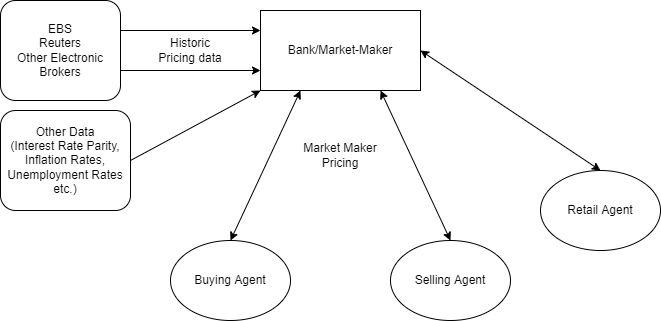
\includegraphics[scale=0.6]{model_architecture.png}
  \caption{Agent Based Model Design}
  \label{fig:model}
\end{figure}


The mechanism in which the market-maker will determine an exchange rate depends on a number of factors. Each market-maker in reality will have a different way of calculating this rate and will apply their own margins accordingly to service their clients. For this model, all market makers will use the same method to determine the exchange rate, but will be given some variance factors that will make each bank in the model have different rates at different times. The change in exchange rate for the model will be made up of the interest rate parity, the money supply of the given currency and the inflation rates and unemployment data for each country. This can be given as the following: $\Delta R_t = f(i, m, x) + \mu _t$ where $\Delta R_t$ is the change in exchange rate, $f$ is a function that is applied to the given data to transform it into the given exchange rate for a market-maker. $i$ is the interest rate parity, $m$ is the money supply, $x$ is the other macro-economic factors such as unemployment data, inflation rate, etc. $\mu _t$ is the residual noise term to lead to a stable model that reaches an equilibrium quickly. \cite{delage2011multi}





%\chapter{Report Body}
The central part of the report usually consists of three or four chapters detailing the technical work undertaken during the project. {\bf{\textcolor{red}{The structure of these chapters is highly project dependent}}}. They can reflect the chronological development of the project, e.g. design, implementation, experimentation, optimisation, evaluation, etc (although this is not always the best approach). However you choose to structure this part of the report, you should make it clear how you arrived at your chosen approach in preference to other alternatives. In terms of the software that you produce, you should describe and justify the design of your programs at some high level, e.g. using OMT, Z, VDL, etc., and you should document any interesting problems with, or features of, your implementation. Integration and testing are also important to discuss in some cases. You may include fragments of your source code in the main body of the report to illustrate points; the full source code is included in an appendix to your written report.

\section{Section Heading}

\subsection{Subsection Heading}
\chapter{Design \& Specification}

\section{Design}

As referenced in figure \ref{fig:model}, the ABM will consist of bank agents representing the market-makers and some different types of trading agents that are connected to it as well as some retail traders. Data is fed to the bank agents to determine an exchange rate and and this is observable to the traders who can then act on the rate and trade accordingly.

The model should hence produce a reasonable simulation of the forex market and with more trading activity a trend for the exchange rate for EUR/USD will be produced by the market-makers in the model. From this graph of exchange rate over time, I can compare it to historic data of exchange rates over time. I can then look at the two graphs and use statistical analysis such as the product moment correlation coefficient (PMCC) to determine the correlation between the historic data and the model's output.

\subsection{Model Design}
The model will most likely consist of a very basic environment for agents to exist in. It will be an array of agents in the model's scheduler. Agents should be activated in a random order for each model step to be fair in an ideal sense, however any trades that a bank makes or a bank's traders make will be executed first. This is to reflect the fact that the inter-bank market is a faster market primarily governed by algorithmic trading with around 92\% of trading in the FX market performed by trading algorithms. \cite{kissell2020algorithmic}

\subsection{Agent Design}
Agents will be given different trading functions dependent on what type of agent they are. Bank agents will prioritise minimising risk and will trade higher volumes at lower yields to service its clients. Trading agents such as the buy and sell agents belonging to the banks may want to see higher risk trading opportunities. Retail agents may take on even greater risk to match their higher profit incentive, and may also act in a random manner at times to attempt to mirror the human aspect of retail traders. All agents do not have to trade at every model time step, they can hold long positions if they choose.

\section{Specification}

\subsection{Development Environment}
The Mesa library for Python 3 was chosen as the development package of choice as it comes with ABM data collection built into the library as well as agent scheduling. This means that the basic structure of an agent based model can be built very quickly with some minimal boilerplate code. Furthermore, a front end web server is available for mode visualisation in the form of graphs and histograms etc. It also allows for custom data visualisation components to be built for the web server through JavaScript and allows for fully custom agent behaviour through each step of the model.

\subsection{Front End Specifications}
The Mesa library already provides a front end application for users to view the output of the model and step through each iteration. 
\begin{itemize}
\item The project should aim to provide a clear visual output from the model that shows the exchange rate against time on a line graph for each individual market maker in the model.
\item Options should be available for users to average the market-maker exchange rates and compare the model output to historic data available.
\item The front end should be able to display metrics about differences in average yield between different types of trading agents as well as profit distribution.
\end{itemize} 


\subsection{Agent Specifications}
\begin{itemize}
\item The Agent should provide intelligent mechanisms to use when trading with a market-maker.
\item The market-makers should have statistically sound and consistent internal functions for calculating the exchange rate at each time step from the given data.
\end{itemize}

\subsection{Model Specifications}
\begin{itemize}
\item The model should provide a suitable environment for agents to interact with one another, whether it be a grid or an array for the agents to reside in. The likely choice will be an array for agents to be placed into as movement does not need to be modelled.
\item The model should provide an appropriately fair activation schedule for the agents to accurately simulate the FX market. Random activation on the schedule for each model step seems appropriately fair for all agents in the model. A distribution for traders trading with the bank to be activated first may be a more realistic approach and will be considered.
\item The model should provide data collection tools to produce a model output to be visualised.
\end{itemize}

%\chapter{Implementation}

\section{Section Heading}

%\chapter{Legal, Social, Ethical and Professional Issues}
Your report should include a chapter with a reasoned discussion about legal, social ethical and professional issues within the context of your project problem. You should also demonstrate that you are aware of the regulations governing your project area and the Code of Conduct \& Code of Good Practice issued by the British Computer Society, and that you have applied their principles, where appropriate, as you carried out your project.

\section{Section Heading}

%\chapter{Results/Evaluation}

\section{Software Testing}

\section{Section Heading}

%\chapter{Conclusion and Future Work}

The project's conclusions should list the key things that have been learnt as a consequence of engaging in your project work. For example, ``The use of overloading in C++ provides a very elegant mechanism for transparent parallelisation of sequential programs'', or ``The overheads of linear-time n-body algorithms makes them computationally less efficient than $O(n \log n)$ algorithms for systems with less than 100000 particles''. Avoid tedious personal reflections like ``I learned a lot about C++ programming...'', or ``Simulating colliding galaxies can be real fun...''. It is common to finish the report by listing ways in which the project can be taken further. This might, for example, be a plan for turning a piece of software or hardware into a marketable product, or a set of ideas for possibly turning your project into an MPhil or PhD.

%%%%%%%%%%%%%%%%%%%%%%%%%%%%%%%%%
% References
%%%%%%%%%%%%%%%%%%%%%%%%%%%%%%%%%
\bibliographystyle{plain}
\bibliography{references}
\addcontentsline{toc}{section}{References}
%%%%%%%%%%%%%%%%%%%%%%%%%%%%%%%%%
% Appendices
%%%%%%%%%%%%%%%%%%%%%%%%%%%%%%%%%
\appendix
%\include{Appendices/appendix}
%\chapter{User Guide}
\section{Instructions}
You must provide an adequate user guide for your software. The guide should provide easily understood instructions on how to use your software. A particularly useful approach is to treat the user guide as a walk-through of a typical session, or set of sessions, which collectively display all of the features of your package. Technical details of how the package works are rarely required. Keep the guide concise and simple. The extensive use of diagrams, illustrating the package in action, can often be particularly helpful. The user guide is sometimes included as a chapter in the main body of the report, but is often better included in an appendix to the main report.

%\chapter{Source Code}
\section{Instructions}
Complete source code listings must be submitted as an appendix to the report. The project source codes are usually spread out over several files/units. You should try to help the reader to navigate through your source code by providing a ``table of contents'' (titles of these files/units and one line descriptions). The first page of the program listings folder must contain the following statement certifying the work as your own: ``I verify that I am the sole author of the programs contained in this folder, except where explicitly stated to the contrary''. Your (typed) signature and the date should follow this statement.

All work on programs must stop once the code is submitted to KEATS. You are required to keep safely several copies of this version of the program and you must use one of these copies in the project examination. Your examiners may ask to see the last-modified dates of your program files, and may ask you to demonstrate that the program files you use in the project examination are identical to the program files you have uploaded to KEATS. Any attempt to demonstrate code that is not included in your submitted source listings is an attempt to cheat; any such attempt will be reported to the KCL Misconduct Committee.

\textbf{You may find it easier to firstly generate a PDF of your source code using a text editor and then merge it to the end of your report. There are many free tools available that allow you to merge PDF files.}


\end{document}
